%!TEX encoding = UTF-8 Unicode
%!TeX spellcheck = en-US
\documentclass[11pt]{article}
\usepackage[utf8]{inputenc}
\usepackage[T1]{fontenc}
\usepackage[hmargin=1in,vmargin=1in]{geometry}

\usepackage{graphicx,wrapfig}
\DeclareGraphicsExtensions{.pdf,.png,.jpg}
\graphicspath{{fig/}}

%\usepackage[charter]{mathdesign}
%\usepackage{berasans,beramono}
\usepackage{microtype}
\usepackage{lmodern}

\usepackage{hyperref}
\hypersetup{colorlinks=true, urlcolor=Blue, citecolor=Green, linkcolor=BrickRed, breaklinks, unicode}

\usepackage[dvipsnames,usenames]{xcolor}
\usepackage[nocompress]{cite}
\usepackage{amsmath,mathtools,stmaryrd}
\usepackage[shortlabels]{enumitem}

% \renewcommand\theenumi{\arabic{enumi}}
% \renewcommand\labelenumi{\theenumi.}
%
% \renewcommand\theenumii{\Alph{enumii}}
% \renewcommand\labelenumii{\theenumii}
%
% \renewcommand\theenumiii{\roman{enumiii}}
% \renewcommand\labelenumiii{\theenumiii.}
%
% \renewcommand\theenumiv{(\alph{enumiv})}
% \renewcommand\labelenumiv{\theenumiv}

\usepackage{arydshln}

\usepackage{todonotes}
\def\etal{\emph{et~al.}}

\dashlinedash 0.75pt
\dashlinegap 1.5pt

\usepackage{latexsym,amsmath,amsthm}
\usepackage{amssymb,stmaryrd}

\usepackage{mathtools} % for \coloneqq

\usepackage{pifont} % for flower
%\usepackage{mathapx} % for rip

% \usepackage{etoolbox}
% \makeatletter
% \setbool{@fleqn}{false}
% \makeatother

\def\etal{\textit{et~al.}}
\def\poly{\mathop{\mathrm{poly}}}
\def\polylog{\mathop{\mathrm{polylog}}}
\def\eps{\varepsilon}
\def\softO{\widetilde{O}}
\def\bd{{\partial}}
\def\reals{\mathbb{R}}
\def\ints{\mathbb{Z}}
\DeclareMathOperator*{\argmax}{arg\,max}
\DeclareMathOperator*{\argmin}{arg\,min}

% ---- DELIMITER PAIRS ----
\def\floor#1{\lfloor #1 \rfloor}
\def\ceil#1{\lceil #1 \rceil}
\def\seq#1{\langle #1 \rangle}
\def\set#1{\{ #1 \}}
\def\abs#1{\mathopen| #1 \mathclose|}		% use instead of $|x|$
\def\norm#1{\mathopen\| #1 \mathclose\|}	% use instead of $\|x\|$
\def\indic#1{\big[#1\big]}			% indicator variable; Iverson notation
							% e.g., Kronecker delta = [x=0]

% --- Self-scaling delmiter pairs ---
\def\Floor#1{\left\lfloor #1 \right\rfloor}
\def\Ceil#1{\left\lceil #1 \right\rceil}
\def\Seq#1{\left\langle #1 \right\rangle}
\def\Set#1{\left\{ #1 \right\}}
\def\Abs#1{\left| #1 \right|}
\def\Norm#1{\left\| #1 \right\|}
\def\Paren#1{\left( #1 \right)}		% need better macro name!
\def\Brack#1{\left[ #1 \right]}		% need better macro name!
\def\Indic#1{\left[ #1 \right]}		% indicator variable; Iverson notation

\def\tsupply{\phi}
\def\fsupply{\phi}

\def\arcto{\mathord\shortrightarrow}
\def\arc#1#2{#1\arcto#2}

\def\Refine{\textsc{Refine}}
\def\Update{\textsc{Update}}

%\def\cost{\operatorname{cost}}
\def\cost{c}
\def\parent{\operatorname{par}}
\def\short{\operatorname{short}}
\def\supp{\operatorname{supp}}
\def\intracount{\operatorname{count}}

\def\alive#1{{#1}^\text{\ding{96}}}
\def\dead#1{{#1} \setminus \alive{#1}}
%\def\dead#1{{#1}^\text{\ding{61}}}
\def\star{\text{\ding{84}}}


%\theoremstyle{plain}
\newtheorem{lemma}{Lemma}[section]
\newtheorem{theorem}[lemma]{Theorem}
\newtheorem{corollary}[lemma]{Corollary}
%\newtheorem{observation}[lemma]{Observation}
%\newtheorem{claim}[lemma]{Claim}
%\newtheorem{definition}[lemma]{Definition}
\numberwithin{figure}{section}


% for definitions
%\definecolor{DarkRed}{rgb}{0.50,0.00,0.00}
\def\EMPH#1{\textcolor{BrickRed}{{\emph{#1}}}}
%\def\EMPH#1{\textbf{\boldmath #1}}
%\def\EMPH#1{\textbf{\emph{\boldmath #1}}}
\pdfstringdefDisableCommands{\let\boldmath\relax} % allow \boldmath in section titles

% ----------------------------------------------------------------------
%  Notes to myself.  The margin flags are broken, thanks to an
%  incompatibility with the geometry package.
% ----------------------------------------------------------------------
\def\n@te#1{\textsf{\boldmath \textbf{$\langle\!\langle$#1$\rangle\!\rangle$}}\leavevmode}
\def\note#1{\textcolor{red}{\n@te{#1}}}
%\renewcommand{\note}[1]{} % use to clear notes


%----------------------------------------------------------------------
% 'cramped' list style, stolen from Jeff Vitter.  Doesn't always work.
%----------------------------------------------------------------------
\def\cramped
  {\parskip\@outerparskip\@topsep\parskip\@topsepadd2pt\itemsep0pt
}

% adding references to description environment; used for representing invariant
\makeatletter
\def\namedlabel#1#2{\begingroup
    #2%
    \def\@currentlabel{#2}%
    \phantomsection\label{#1}\endgroup
}


%% METAFILE
\title{Efficient Algorithms for Geometric Partial Matching%
\date{\today} % replace with date?
\author{
Pankaj K.\ Agarwal
\and
Hsien-Chih Chang
\and
Allen Xiao
}
}

%\title{Efficient Algorithms for Geometric Partial Matching}
%\titlerunning{Efficient Algorithms for Geometric Partial Matching}
%\author{Pankaj K.\ Agarwal}{Duke University, Durham, USA}{pankaj@cs.duke.edu}{}{}
%\author{Hsien-Chih Chang}{Duke University, Durham, USA}{hsienchih.chang@duke.edu}{}{}
%\author{Allen Xiao}{Duke University, Durham, USA}{axiao@cs.duke.edu}{}{}
%\date{\today}

%\authorrunning{P.\ K.\ Agarwal, H.-C.\ Chang, A.\ Xiao}
%\Copyright{Pankaj K.\ Agarwal, Hsien-Chih Chang, Allen Xiao}

%\ccsdesc{Theory of computation~Design and analysis of algorithms}
%\keywords{partial matching, transportation, optimal transport, minimum-cost flow, bichromatic closest pair}
%\acknowledgements{
%We thank Haim Kaplan for discussion and suggestion to use
%Goldberg~\etal~\cite{GHKT17} algorithm.
%We thank Debmalya Panigrahi for helpful discussions.
%}
%\funding{
%Work on this paper was supported by NSF under grants CCF-15-13816,
%CCF-15-46392, and IIS-14-08846, by an ARO grant W911NF-15-1-0408, and by
%BSF Grant 2012/229 from the U.S.-Israel Binational Science Foundation.
%}
%\relatedversion{A full version of this paper is available at \url{XXX}}

%\EventEditors{Gill Barequet and Yusu Wang}
%\EventNoEds{2}
%\EventLongTitle{35th International Symposium on Computational Geometry (SoCG 2019)}
%\EventShortTitle{SoCG 2019}
%\EventAcronym{SoCG}
%\EventYear{2019}
%\EventDate{June 18--21, 2019}
%\EventLocation{Portland, Oregon, USA}
%\EventLogo{socg-logo}
%\SeriesVolume{129}
%\ArticleNo{6}


\begin{document}

\maketitle

\begin{abstract}
Let $A$ and $B$ be two point sets in the plane of sizes $r$ and $n$ respectively (assume $r \leq n$), and let $k$ be a parameter.
A matching between $A$ and $B$ is a family of pairs in $A \times B$ so that any point of $A \cup B$ appears in at most one pair.
Given two positive integers $p$ and $q$, we define the cost of matching $M$ to be $\cost(M) = \sum_{(a, b) \in M}\norm{a-b}_p^q$ where $\norm{\cdot}_p$ is the $L_p$-norm.
The geometric partial matching problem asks to find the minimum-cost size-$k$ matching between $A$ and $B$.

We present efficient algorithms for geometric partial matching problem that work for any powers of $L_p$-norm matching objective:
An exact algorithm that runs in $O((n + k^2)\polylog n)$ time, and a $(1 + \eps)$-approximation algorithm that runs in $O((n + k\sqrt{k})\polylog n \cdot \log\eps^{-1})$ time.
Both algorithms are based on the primal-dual flow augmentation scheme; the main improvements involve using dynamic data structures to achieve efficient flow augmentations.
With similar techniques, we give an exact algorithm for the planar transportation problem running in $O(\min\{n^2, rn^{3/2}\}\polylog n)$ time.
\end{abstract}


% ----------------------------------------------------------------------------
\section{Introduction}

Given two point sets $A$ and $B$ in the plane, we consider the problem of finding
the minimum-cost partial matching between $A$ and $B$.
Formally, suppose $A$ has size $r$ and $B$ has size $n$ where $r \leq n$.
Let $G(A, B)$ be the undirected complete bipartite graph between
$A$ and $B$, and let the cost of edge $(a, b)$ be
$\EMPH{$c(a, b)$} = \norm{a-b}_p^q$, for some positive integers $p$ and $q$.
%Define $\EMPH{$C$} \coloneqq \max_{(a, b) \in A \times B} c(a, b)$.
A \EMPH{matching} $M$ in $G(A, B)$ is a set of edges sharing no endpoints.
The \EMPH{size} of $M$ is the number of edges in $M$.
The cost of matching $M$, denoted \EMPH{$\cost(M)$}, is defined to be the sum of costs of edges in $M$.
For a parameter $k$, the problem of finding the minimum-cost
size-$k$ matching in $G(A, B)$ is called the \EMPH{geometric partial matching problem}.
We call the corresponding problem in general bipartite graphs (with arbitrary
edge costs) the \EMPH{partial matching problem}.%
\footnote{Partial matching is also called \EMPH{imperfect matching} or \EMPH{imperfect assignment} \cite{RT12,GHKT17}.}

We also consider the following generalization of bipartite matching.
Let $\tsupply:A \cup B \to \ints$ be an integral \EMPH{supply-demand function} with
positive value on points of $A$ and negative value on points of $B$, satisfying
$\sum_{a \in A} \tsupply(a) = - \sum_{b \in B} \tsupply(b)$.
Let $\EMPH{$U$} \coloneqq \max_{p \in A \cup B} \abs{\tsupply(p)}$.
A \EMPH{transportation map} is a function $\tau: A \times B \to \reals_{\geq 0}$
such that $\sum_{b \in B} \tau(a, b) = \tsupply(a)$ for all $a \in A$ and
$\sum_{a \in A} \tau(a, b) = -\tsupply(b)$ for all $b \in B$.
We define the cost of $\tau$ to be
\begin{equation*}
	\EMPH{$\cost(\tau)$} \coloneqq \sum_{(a, b) \in A \times B} c(a, b) \cdot \tau(a, b).
\end{equation*}
The \EMPH{transportation problem} asks to compute a transportation map of minimum cost.

%Both matching and transportation problems arise in a broad range of applications,
%for example, in
%computer vision and graphics~\cite{RTG98,SGPCBNDG15,P15},
%machine learning~\cite{BBR06,ACB17},
%economics~\cite{G16},
%engineering~\cite{STTP14},
%and medical imaging~\cite{GPC15}.
%More recently, computational/numerical interest has expanded greatly due to
%the development of fast approximate solvers \cite{C13,AWR17,DGK18};
%see the books by Villani~\cite{V03,V08}, by Cuturi and Peyr{\'e}~\cite{PC18},
%and the survey by Solomon~\cite{S18}.

\paragraph*{Related work.}
Maximum-size bipartite matching is a classical problem in graph algorithms.
Upper bounds include the $O(m\sqrt{n})$ time algorithm by
Hopcroft and Karp~\cite{HK73} and the $O(m \min\{\sqrt{m}, n^{2/3}\})$ time
algorithm by Even and Tarjan~\cite{ET75}, where $n$ is the
number of nodes and $m$ is the number of edges.
The first improvement in over thirty years was made by M{\k a}dry~\cite{M13},
which uses an interior-point algorithm, runs in $O(m^{10/7}\polylog n)$ time.

The Hungarian algorithm~\cite{Kuhn55} computes a minimum-cost maximum matching
in a bipartite graph in roughly $O(mn)$ time.
Faster algorithms have been developed,
%for minimum-weight bipartite matching,
such as the $O(m\sqrt{n}\log(nC))$ time algorithms by Gabow and
Tarjan~\cite{GT89} and the improved $O(m\sqrt{n}\log C)$ time algorithm by
Duan~\etal~\cite{DPS18} assuming the edge costs are integral;
here $C$ is the maximum cost of an edge.
Ramshaw and Tarjan~\cite{RT12} showed that the Hungarian algorithm can be extended to compute a minimum-cost partial
matching of size $k$ in $O(km + k^2\log r)$ time, where $r$ is the size of the smaller side of the bipartite graph.
They also proposed a cost-scaling algorithm for partial
matching that runs in time $O(m\sqrt{k}\log(kC))$, again assuming that costs
are integral.
By reduction to unit-capacity min-cost flow, Goldberg~\etal~\cite{GHKT17}
developed a cost-scaling algorithm for partial matching with an identical running time
$O(m\sqrt{k}\log(kC))$,
%$= O(nr\sqrt{k}\log(kC))$
again only for integral edge costs.

In geometric settings, the Hungarian algorithm can be implemented to compute
an optimal perfect matching between $A$ and $B$ (assuming equal size)
in time $O(n^2\polylog n)$~\cite{KMRSS17} (see also \cite{Vaidya89,AES99}).
This algorithm computes an optimal size-$k$ matching in time $O(kn\polylog n)$.
Faster approximation algorithms have been developed for computing perfect
matchings in geometric settings \cite{Vaidya89,V98,AV04,SA12}.
Recall that the cost of the edges are the $q$th power of their $L_p$-distances.
When $q = 1$, the best algorithm to date by Sharathkumar and Agarwal~\cite{SA12m}
computes $(1+\eps)$-approximation to the value of optimal perfect matching in
$O(n\polylog n \cdot \poly\eps^{-1})$ expected time with high probability.
Their algorithm can also compute a $(1+\eps)$-approximate partial
matching within the same time bound.
For $q > 1$, the best known approximation algorithm to compute a perfect
matching runs in $O(n^{3/2}\polylog n \log(1/\eps))$ time \cite{SA12};
it is not obvious how to extend this algorithm to the partial matching setting.

The transportation problem can also be formulated as an instance of the
minimum-cost flow problem.
The strongly polynomial uncapacitated min-cost flow algorithm by
Orlin~\cite{O93} solves the transportation problem in
$O((m + n\log n) n\log n)$ time.
Lee and Sidford~\cite{LS14} give a weakly polynomial algorithm that runs in
$O(m\sqrt{n}\polylog(n, U))$ time, where $U$ is the maximum amount of node supply-demand.
Agarwal~\etal~\cite{AFPVX17, AFPVX17arxiv} showed that Orlin's algorithm can be
implemented to solve 2D transportation in time $O(n^2\polylog n)$.
In case of $O(1)$-dimension Euclidean space,
by adapting the Lee-Sidford algorithm, they developed a
$(1+\eps)$-approximation algorithm that runs in $O(n^{3/2} \poly\eps^{-1} \polylog(n, U))$ time.
They also gave a Monte-Carlo algorithm that computes an
$O(\log^2(1/\eps))$-approximate solution in $O(n^{1+\eps})$ time with
high probability.
Recently, Khesin, Niklov, and Paramonov~\cite{KNP19} obtained a
$(1+\eps)$-approximation in low-dimensional Euclidean space
that runs in randomized $O(n \poly\eps^{-1} \polylog(n, U))$ time. %TODO explain more once we know

\paragraph*{Our results.}
There are three main results in this paper.
First in Section~\ref{section:hung} we present an efficient algorithm for
computing an optimal partial matching in the plane.

\begin{theorem}
\label{theorem:hung}
Given two point sets $A$ and $B$ in the plane each of size at most $n$ and an
integer $k \leq n$, a minimum-cost matching of size $k$ between $A$ and $B$ can
be computed in $O((n + k^2)\polylog n)$ time.
\end{theorem}

We use \emph{bichromatic closest pair (BCP)} data structures to implement the Hungarian algorithm efficiently, similar to Agarwal~\etal~\cite{AES99} and Kaplan~\etal~\cite{KMRSS17}.
But unlike their algorithms which take $\Omega(n)$ time to find an
augmenting path, we show that after $O(n\polylog n)$ time preprocessing,
an augmenting path can be found in $O(k\polylog n)$ time.
The key is to recycle (rather than rebuild) our data structures from one
augmentation to the next.
We refer to this idea as the \emph{rewinding mechanism}.
%and it will be used in our other algorithms as well.

\medskip

Next in Sections~\ref{section:goldberg},
we obtain a $(1+\eps)$-approximation algorithm for the geometric partial
matching problem in the plane by providing an efficient implementation of the
unit-capacity min-cost flow algorithm by Goldberg~\etal~\cite{GHKT17}.

\begin{theorem}
\label{theorem:gmcm}
Given two point sets $A$ and $B$ in $\reals^2$ each of size at most $n$,
an integer $k \leq n$, and a parameter $\eps > 0$, a $(1+\eps)$-approximate
min-cost matching of size $k$ between $A$ and $B$ can be computed in
$O((n + k\sqrt{k})\polylog n \cdot \log\eps^{-1})$ time.
\end{theorem}

The main challenge here is how to deal with the \emph{dead nodes},
which neither have excess/deficit nor have flow passing through them,
but still contribute to the size of the graph.
We show that the number of \emph{alive nodes} is only $O(k)$, and then
represent the dead nodes implicitly so that the Hungarian search and
computation of a blocking flow can be implemented in $O(k\polylog n)$ time.

\medskip

Finally in Section~\ref{section:orlin} we present a faster algorithm for the
transportation problem in $\reals^2$ when the two point sets are unbalanced.

\begin{theorem}
\label{theorem:orlin}
Given two point sets $A$ and $B$ in $\reals^2$ of sizes $r$ and $n$ respectively
with $r \leq n$, along with supply-demand function $\tsupply:A \cup B \to \ints$,
an optimal transportation map between $A$ and $B$ can be computed in
$O(\min\{n^2, rn^{3/2}\}\polylog n)$ time.
\end{theorem}

Our result improves over the $O(n^2\polylog n)$ time algorithm by Agarwal
\etal~\cite{AFPVX17arxiv} for $r = o(\sqrt{n})$.
Similar to their algorithm, we also use the strongly polynomial uncapacitated
minimum-cost flow algorithm by Orlin~\cite{O93}, but additional ideas are
needed for efficient implementation.
%\note{``If needed, we can remove this part.''}
Unlike in the case of matchings, the support of the transportation problem may
have size $\Omega(n)$ even when $r$ is a constant;
so na\"ively we can no longer spend time proportional to the size of
support of the transportation map.
However, with careful implementation we ensure that the support is acyclic,
and one can find an augmenting path in $O(r\sqrt{n} \polylog n)$ time with
proper data structures, assuming $r \leq \sqrt{n}$.
%\note{Do we need this condition for data structures?}


% ----------------------------------------------------------------------------
\section{Minimum-cost partial matchings using Hungarian algorithm}
\label{section:hung}

% The Hungarian algorithm~\cite{Kuhn55} is a primal-dual algorithm for min-cost
% bipartite matching in general graphs that can be adapted to solve the partial matching problem exactly if
% one terminates the algorithm after $k$ iterations (see e.g.~\cite{RT12}).
In this section, we solve the geometric partial matching problem and prove Theorem~\ref{theorem:hung} by implementing the Hungarian algorithm for partial matching in $O((n + k^2)\polylog n)$ time.

%\subsection{Matching Terminologies}

% \note{Move some to intro}
% Let $G$ be a bipartite graph between node sets $A$ and $B$ and edge set $E$,
% with costs $c(v, w)$ for each edge $(v, w)$ in $G$.
% A \EMPH{matching} $M \subseteq E$ is a set of edges where no two edges share an
% endpoint.
% A node $v$ is \EMPH{matched} by $M$ if $v$ is the endpoint of some matching edge in $M$;
% otherwise $v$ is \EMPH{unmatched}.
% %We use $V(M)$ to denote the nodes matched by $M$.
% The \EMPH{size} of a matching is the number of edges in the set, and the
% \EMPH{cost} of a matching is the sum of costs of its edges.
% For a parameter $k$, the \EMPH{minimum-cost partial matching problem (MPM)}
% asks to find a size-$k$ matching of minimum cost.
% In the geometric partial matching setting, we have $E = A \times B$
% and $c(a, b) = \norm{a-b}_p^q$ for every edge $(a, b)$ in $G$.

A node $v$ is \EMPH{matched} by matching $M$ if $v$ is the endpoint of some edge in $M$;
otherwise $v$ is \EMPH{unmatched}.
Given a matching $M$, an \EMPH{augmenting path}
$\Pi = (a_1, b_1, \ldots, a_\ell, b_\ell)$ is an odd-length path with unmatched
endpoints ($a_1$ and $b_\ell$) that alternates between edges outside and inside of $M$.
The symmetric difference $M \oplus \Pi$ creates a new matching of size $\abs{M}+1$, called the \EMPH{augmentation} of $M$ by $\Pi$.
%
The dual to the standard linear program for partial matching has one dual variable
for each node $v$, called the \EMPH{potential $\pi(v)$} of $v$.
Given potential $\pi$, we can define the \EMPH{reduced cost} of the edges to be
$\EMPH{$c_\pi(v, w)$} \coloneqq c(v, w) - \pi(v) + \pi(w)$.
Potential $\pi$ is \EMPH{feasible} on edge $(v,w)$ if $c_\pi(v, w)$ is nonnegative.
Potential $\pi$ is \EMPH{feasible} if $\pi$ are feasible on every edge in $G$.
We say that an edge $(v, w)$ is \EMPH{admissible} under potential $\pi$ if $c_\pi(v, w) = 0$.

\paragraph*{Fast implementation of Hungarian search.}

The Hungarian algorithm is initialized with $M \gets \emptyset$ and $\pi \gets 0$.
% It maintains the following invariants: (see, for example, \cite{})
% %\begin{enumerate}[(i)]\itemsep=0pt
% (i) $\pi$ is feasible,
% (ii) all edges in $M$ are admissible,
% (iii) unmatched nodes of $A$ all have the same potential $\alpha$ satisfying $\alpha \geq \pi(a)$ for any matched node $a \in A$, and
% (iv) unmatched nodes of $B$ all have the same potential $\beta$ satisfying $\beta \leq \pi(b)$ for any matched node $b \in B$.
% %\end{enumerate}
% Ramshaw and Tarjan~\cite{RT12} show that these conditions are sufficient to
% guarantee that $M$ is a minimum-cost matching.
Each iteration of the Hungarian algorithm augments $M$ by an admissible
augmenting path $\Pi$, discovered using a procedure called the
\EMPH{Hungarian search}.
The algorithm terminates after $k$ augmentations, exactly when $\abs{M} = k$;
Ramshaw and Tarjan~\cite{RT12} showed that $M$ is guaranteed to be an optimal partial matching.
%\note{For the specific implementation of Hungarian search where in each iteration the roots are all unmatched nodes in $A$.  Picking one as source does not guarantee min-cost partial matching.}

The Hungarian search grows a set of \EMPH{reachable nodes $X$} from
all unmatched $v \in A$ using augmenting paths of admissible edges.
Initially, $X$ is the set of unmatched nodes in $A$.
Let the \EMPH{frontier} of $X$ be the edges in $(A \cap X) \times (B \setminus X)$.
$X$ is grown by \EMPH{relaxing} an edge $(a, b)$ in the frontier:
Add $b$ into $X$, modify potential to make $(a, b)$ admissible,
preserve $c_\pi$ on other edges within $X$, and keep $\pi$ feasible on edges outside of $X$.
Specifically, the algorithm relaxes the min-reduced-cost frontier edge $(a, b)$,
and then raises $\pi(v)$ by $c_\pi(a, b)$ for all $v \in X$.
%It is easy to verify that this potential change preserves feasibility.
%
% \note{Compress details...}
% As $b \in B$ is added into $X$, we can store a backpointer to $a$, which can be
% used later to recover the admissible augmenting path through $b$.
% If $b$ is matched, say to node $a'$, then we also relax $(a', b)$ by adding $a'$
% into $X$ (no potential change needed, by invariant) with backpointer to $b$.
% If $b$ is unmatched, the search finishes and we can recover an admissible
% augmenting path to $b$ by following backpointers to an unmatched node $a \in A$.
% %Once $X$ contains an unmatched $b \in B$, an admissible augmenting path exists.
% \note{... to here.}
If $b$ is already matched, then we also relax the matching edge $(a',b)$ and add $a'$ into $X$.
The search finishes when $b$ is unmatched, and an admissible augmenting path now can be recovered.

%Each augmenting path has length $O(k)$, as every other edge is a matching edge and $|M| \leq k$. \note{not needed here?}
%Additionally, there are $k$ augmentations throughout the Hungarian algorithm.
%so the total time spent on updating the matching (during augmentations) is $O(k^2)$.

%\subsection{Fast implementation of Hungarian search}
%\label{SS:fast-hungarian-matching}

% Observe that the Hungarian search makes $O(k)$ relaxations, as each
% relaxation either leads to an unmatched node (ending the search) or
% adds both nodes of a matching edge.
% We will implement each relaxation step in $O(\polylog n)$ time, after
% preprocessing.

%In general graphs,
%The most expensive step in augmentation is to find the minimum-reduced-cost frontier edge that needs to be relaxed --- the search must ``look at every edge''.
%e.g.\ by pushing them into a priority queue even if they are not relaxed.
In the geometric setting, we find the min-reduced-cost frontier edge using a dynamic
\EMPH{bichromatic closest pair} (BCP) data structure, similar to \cite{AFPVX17arxiv,Vaidya89}.
Given two point sets $P$ and $Q$ in the plane and a weight function
$\omega: P\cup Q \to \reals$, the BCP is two points $a \in P$ and $b \in Q$
minimizing the additively weighted distance $c(a, b) - \omega(a) + \omega(b)$.
Thus, a minimum reduced-cost frontier edge is precisely the BCP of point sets
$P = A \cap X$ and $Q = B \setminus X$, with $\omega = \pi$.
Note that the ``state'' of this BCP is parameterized by $X$ and $\pi$.

%\note{Short history on BCP?}
%\note{Under the assumption ... on the metric,}
The dynamic BCP data structure by Kaplan \etal~\cite{KMRSS17} supports point insertions and deletions in
$O(\polylog n)$ time and answers queries in $O(\log^2 n)$ time for our setting.
Each relaxation in the Hungarian search requires
one query, one deletion, and at most one insertion (aside from the potential updates).
As $\abs{M} \leq k$ throughout, there are at most $2k$ relaxations in each
Hungarian search, and the BCP can be used to implement each Hungarian search
in $O(k\polylog n)$ time.
%Explained shortly, there is an existing technique to handle potential updates
%without performing BCP updates for each one \note{?}.

\paragraph*{Rewinding mechanism.}
% In the beginning of each iteration,
% $X$ is initialized to the set of unmatched nodes in $A$,
% and therefore $Q = B \setminus X$ has size $n$.
We observe that exactly one node of $A$ is newly matched after an augmentation.
Thus (modulo potential changes), we can obtain the initial state of the BCP for
the $(i+1)$-th Hungarian search from the $i$-th one with a single BCP deletion.

If we remember the sequence of points added to $X$ in the $i$-th Hungarian search,
then at the start of the $(i+1)$-th Hungarian search we can \emph{rewind} this
sequence by applying the opposite insert/delete operation to each BCP update
in reverse order to obtain the initial state of the $i$-th BCP.
With one additional BCP deletion, we have the initial state of the $(i+1)$-th BCP.
The number of insertions/deletions is bounded by the number of
relaxations per Hungarian search which is $O(k)$.
Therefore we can recover, in $O(k\polylog n)$
time, the initial BCP data structure for each Hungarian search beyond the first.
We refer to this procedure as the \EMPH{rewinding mechanism}.

%\begin{lemma}
%\label{L:fast-hungarian}
%Each Hungarian search can be implemented
%in $O(k\polylog n)$ time after a one-time $O(n\polylog n)$ preprocessing.
%\end{lemma}

\paragraph*{Potential updates.}
We modify a trick from Vaidya~\cite{Vaidya89} to batch potential updates.
Potential is tracked with a \EMPH{stored value} $\gamma(v)$, while the
\EMPH{true value} of $\pi(v)$ may have changed since $\gamma(v)$ was last recorded.
This is done by aggregating potential changes into a variable $\EMPH{$\delta$}$,
which is initially 0 at the very beginning of the algorithm.
Whenever we would raise the potential of all nodes in $X$, we raise
$\delta$ by that amount instead.
We maintain the following invariant: $\pi(v) = \gamma(v)$ for $v \not\in X$,
and $\pi(v) = \gamma(v) + \delta$ for $v \in X$.

At the beginning of the algorithm, $X$ is empty and stored values are equal to
true values.
When $a \in A$ is added to $X$, we update its stored value to $\pi(a) - \delta$
for the current value of $\delta$, and use that stored value as its BCP weight.
Since the BCP weights are uniformly offset from $\pi(v)$ by $\delta$, the pair
reported by the BCP is still minimum.
When $b \in B$ is added to $X$, we update its stored value to $\pi(b) - \delta$
(although it won't be added to a BCP set).
When a node is removed from $X$ (e.g.\ by augmentation or rewinding), we update
the stored potential $\gamma(v) \gets \pi(v) + \delta$, again for the current
value of $\delta$.
Unlike Vaidya~\cite{Vaidya89} and for the sake of rewinding, we do not reset $\delta$ across Hungarian searches.

There are $O(k)$ relaxations and thus $O(k)$ updates to $\delta$ per Hungarian search.
$O(k)$ stored values are updated per rewinding, so the time spent on potential
updates per Hungarian search is $O(k)$.
Putting everything together, our implementation of the Hungarian algorithm runs
in $O((n + k^2)\polylog n)$ time.
This proves Theorem~\ref{theorem:hung}.


% ----------------------------------------------------------------------------
\section{Approximating min-cost partial matching through cost-scaling}
\label{section:goldberg}

In this section we describe an approximation algorithm for computing a min-cost
partial matching.
%in the graph $G(A, B)$ defined earlier.
We reduce the problem to computing a min-cost circulation in a flow network
(Section~\ref{SS:match-flow-red}).
We adapt the cost-scaling algorithm by Goldberg~\etal~\cite{GHKT17} for
computing min-cost flow of a unit-capacity network (Section~\ref{SS:cost-scale}).
Finally, we show how their algorithm can be implemented in
$O\Paren{(n + k^{3/2})\polylog(n)\log(1/\eps)}$ time in our setting (Section~\ref{SS:fast_refine}).

\subsection{From matching to circulation}
\label{SS:match-flow-red}

Given a bipartite graph $G$ with node sets $A$ and $B$, we construct a flow network
$N = (V, \vec{E})$ in a standard way \cite{RT12}
so that a min-cost matching in $G$ corresponds to a min-cost integral
circulation in $N$.

\paragraph*{Flow network.}
Each node in $G$ becomes a node in $N$ and each edge
$(a, b)$ in $G$ becomes an arc $\arc{a}{b}$ in $N$;
we refer to these nodes and arcs as \EMPH{bipartite nodes} and \EMPH{bipartite arcs}.
We also include a \EMPH{source} node $s$ and \EMPH{sink} node $t$ in $N$.
For each $a \in A$, we add a \EMPH{left dummy arc} $\arc{s}{a}$ and for each
$b \in B$ a \EMPH{right dummy arc} $\arc{b}{t}$.
The cost \EMPH{$c(\arc{v}{w})$}
%of each arc $\arc{v}{w}$
is equal to $c(v, w)$ if
$\arc{v}{w}$ is a bipartite arc and $0$ if $\arc{v}{w}$ is a dummy arc.
All arcs in $N$ have unit capacity.

Let $\fsupply: V \to \ints$ be an integral supply/demand function on nodes of $N$.
The positive values of $\fsupply(v)$ are referred to as \EMPH{supply}, and the
negative values of $\fsupply(v)$ as \EMPH{demand}.
A \EMPH{pseudoflow} $f: \vec{E} \to [0, 1]$ is a function on arcs of $N$.
The \EMPH{support} of $f$ in $N$, denoted as \EMPH{$\supp(f)$}, is the set of arcs with positive flow.
%$\supp(f) \coloneqq \Set{\arc vw \in \vec{E} \mid f(\arc vw) > 0}$.
Given a pseudoflow $f$, the \EMPH{imbalance} of a node is
\[
\EMPH{$\fsupply_f (v)$} \coloneqq \fsupply(v) + \sum_{\arc wv \in \vec{E}}{f(\arc wv)} - \sum_{\arc vw \in \vec{E}}{f(\arc vw)}.
\]
We call positive imbalance \EMPH{excess} and negative imbalance \EMPH{deficit}.
We refer to the sum of positive imbalance in a pseudoflow as the \EMPH{excess of the pseudoflow}.
A node is \EMPH{balanced} if it has zero imbalance.
If all nodes are balanced, the pseudoflow is a \EMPH{circulation}.
The \EMPH{cost} of a pseudoflow is defined to be
\[
 \EMPH{$\cost(f)$} \coloneqq \sum_{\arc vw \in \supp(f)} c(\arc vw) \cdot f(\arc vw).
\]
The \EMPH{minimum-cost flow problem} (MCF) asks to find a circulation of minimum cost.

If we set $\fsupply(s) = k$, $\fsupply(t) = k$, and $\fsupply(v) = 0$ for all
$v \in A \cup B$, then an integral circulation $f$ corresponds to a partial
matching $M$ of size $k$ and vice versa.
Moreover, $\cost(M) = \cost(f)$.
%
Hence, the problem of computing a min-cost matching of size $k$ in $G$
transforms to computing an integral circulation in $N$.
The following lemma will be useful for our algorithm.

\begin{lemma}
\label{lemma:supp_size}
Let $N$ be the network constructed from the bipartite graph $G$ above.
\begin{enumerate}[(i)]
\item For any integral circulation $g$ in $N$, the size of $\supp(g)$ is at most $3k$.
\item For any integral pseudoflow $f$ in $N$ with $K$ excess,
	the size of $\supp(f)$ is at most $3(K + k)$.
\end{enumerate}
\end{lemma}
\begin{proof}
\begin{enumerate}[(i)]
\item Because $g$ is a circulation, $\supp(g)$ can be decomposed into $k$  paths from $s$ to $t$.
	Each $s$-to-$t$ path in $N$ is of length three, so $\abs{\supp(g)} \leq 3k$.
\item The graph in $N$ is a directed acyclic graph, so $\supp(f)$ does not form a directed cycle.
	Thus, $\supp(f)$ can be decomposed into a set of inclusion-maximal paths,
	each of which contributes a single unit of excess to the flow if the path
	does not terminate at $t$ or if more than $k$ paths terminate at $t$.
	By assumption, there are $K$ units of excess to which we can associate to the paths,
	and at most $k$ paths terminating at $t$ that we cannot associate with a unit of excess.
	Each inclusion-maximal path has length at most 3, so $\abs{\supp(f)} \leq 3(K + k)$.
\end{enumerate}
\end{proof}

\subsection{A cost-scaling algorithm}
\label{SS:cost-scale}

Before describing the algorithm, we need to introduce a few more concepts.

\paragraph*{Residual network and admissibility.}
If $f$ is an integral pseudoflow on $N$
(that is, $f(\arc{v}{w}) \in \{0, 1\}$ for every arc in $\vec{E}$), then each arc
$\arc{v}{w}$ in $N$ is either \EMPH{idle} with $f(\arc{v}{w}) = 0$ or
\EMPH{saturated} with $f(\arc{u}{v}) = 1$.
%\note{define earlier?}

Given a pseudoflow $f$, the \EMPH{residual network} $N_f = (V, \vec{E}_f)$ is
defined as follows.
For each idle arc $\arc{v}{w}$ in $\vec{E}$, we add a \EMPH{forward} residual
arc $\arc{v}{w}$ in $N_f$.
For each saturated arc $\arc{v}{w}$ in $\vec{E}$, we add a \EMPH{backward}
residual arc $\arc{w}{v}$ in $N_f$.
The set of residual arcs in $N_f$ is therefore
\[
\vec{E}_f \coloneqq \{\arc{v}{w} \mid f(\arc{v}{w}) = 0\} \cup \{\arc{w}{v} \mid f(\arc{v}{w}) = 1\}.
\]
The cost of a forward residual arc $\arc{v}{w}$ is $c(\arc{v}{w})$,
while the cost of a backward residual arc $\arc{w}{v}$ is $-c(\arc{v}{w})$.
Each arc in $N_f$ also has unit capacity.
By Lemma~\ref{lemma:supp_size}, $N_f$ has $O(k)$ backward arcs if $f$ has $O(k)$ excess.

A \EMPH{residual pseudoflow} $g$ in $N_f$ can be used to change $f$ into a
different pseudoflow on $N$ by \EMPH{augmentation}.
For simplicity, we only describe augmentation for the case where $f$ and $g$ are integral.
Specifically, augmenting $f$ by $g$ produces a pseudoflow $f'$ in $N$ where
\[
f'(\arc vw) = \begin{cases}
	0 & {\arc wv} \in \vec{E}_f \text{ and } g(\arc wv) = 1, \\
	1 & {\arc vw} \in \vec{E}_f \text{ and } g(\arc vw) = 1, \\
	f(\arc vw) & \text{otherwise.}
\end{cases}
\]

Using LP duality for min-cost flow, we assign \EMPH{potential $\pi(v)$} to each node $v$ in $N$.
The \EMPH{reduced cost} of an arc $\arc{v}{w}$ in $N$ with respect to $\pi$ is
defined as
\[
c_\pi(\arc vw) \coloneqq c(\arc vw) - \pi(v) + \pi(w).
\]
Similarly we define the reduced cost of arcs in $N_f$: the reduced cost of a
forward residual arc $\arc vw$ in $N_f$ is $c_\pi(\arc vw)$, and the reduced cost of a
backward residual arc $\arc wv$ in $N_f$ is $-c_\pi(\arc vw)$.
Abusing the notation, we also use $c_\pi$ to denote the reduced cost of arcs in
$N_f$.
%\note{Unclear.  Does $c_\pi(\arc wv)$ have positive or negative value for a backward arc $\arc wv$?}

The \EMPH{dual feasibility constraint} asks that $c_\pi(\arc vw) \geq 0$ holds
for every arc $\arc vw$ in $\vec{E}$;
potential $\pi$ that satisfy this constraint is said to be \EMPH{feasible}.
Suppose we relax the dual feasibility constraint to allow some small violation
in the value of $c_\pi(\arc vw)$.
We say that a pair of pseudoflow $f$ and potential $\pi$ is
\EMPH{$\theta$-optimal}~\cite{T85,BE87}
%\footnote{This is commonly written as $\eps$-optimality in the min-cost flow literature.}
if $c_\pi(\arc vw) \geq -\theta$ for every residual arc $\arc vw$ in $\vec{E}_f$.
Pseudoflow $f$ is \emph{$\theta$-optimal} if it is $\theta$-optimal with
respect to some potential $\pi$;
potential $\pi$ is \emph{$\theta$-optimal} if it is $\theta$-optimal with
respect to some pseudoflow $f$.
Given a pseudoflow $f$ and potential $\pi$, a residual arc $\arc vw$ in
$\vec{E}_f$ is \EMPH{admissible} if $c_\pi(\arc vw) \leq 0$.
We say that a pseudoflow $g$ in $N_f$ is \EMPH{admissible} if $g(\arc vw) > 0$
only on admissible arcs $\arc vw$, and $g(\arc vw) = 0$ otherwise.%
\footnote{The same admissibility/feasibility definitions will be used later in
	Section~\ref{section:orlin}.
	However, the algorithm in Section~\ref{section:orlin} maintains a
	0-optimal $f$ and therefore admissible residual arcs always have
	$c_\pi(\arc vw) = 0$.}
We will use the following well-known property of $\theta$-optimality.

\begin{lemma}
\label{lemma:eps_opt_preserve}
Let $f$ be an $\theta$-optimal pseudoflow in $N$ and let $g$ be an admissible
pseudoflow in $N_f$.
Then $f$ augmented by $g$ is also $\theta$-optimal in $N$.
\end{lemma}

%\begin{proof}
%Augmentation by $f'$ will not change the potential, so any previously
%$\theta$-optimal arcs remain $\theta$-optimal.
%However, it may introduce new arcs $\arc vw$ with $u_{f+f'}(\arc vw) > 0$, that previously had
%$u_f(\arc vw) = 0$.
%We will verify that these arcs satisfy the $\theta$-optimality condition.
%
%If an arc $\arc vw$ is newly introduced this way, then by definition of residual
%capacities $f(\arc vw) = u(\arc vw)$.
%At the same time, $u_{f+f'}(\arc vw) > 0$ implies that $(f+f')(\arc vw) < u(\arc vw)$.
%This means that $f'$ augmented flow in the reverse direction of $\arc vw$,
%that is, $f'(\arc wv) > 0$.
%By assumption, the arcs of $\supp(f')$ are admissible, so $\arc wv$ was an
%admissible arc ($c_\pi(\arc wv) \leq 0$).
%By antisymmetry of reduced costs, this implies $c_\pi(\arc vw) \geq 0 \geq -\theta$.
%Therefore, all arcs with $u_{f+f'}(v, w) > 0$ respect the $\theta$-optimality condition,
%and thus $f+f'$ is $\theta$-optimal.
%\end{proof}

Using Lemma~\ref{lemma:supp_size}, the following lemma can be proved about
$\theta$-optimality:

\begin{lemma}
\label{lemma:goldberg_cost_add}
Let $f$ be a $\theta$-optimal integer circulation in $N$,
and $f^*$ be an optimal integer circulation for $N$.
Then, $\cost(f) \leq \cost(f^*) + 6k\theta$.
\end{lemma}
\begin{proof}
Taking the symmetric difference between $f$ and $f^*$ gives a residual pseudoflow $g$ of $N_f$,
where augmenting $f$ by $g$ produces $f^*$.
Then, $\cost(f^*) = \cost(f) + \cost(g)$.
Since both $f$ and $f^*$ are circulations, $g$ is comprised of cycle flows in $N_f$.
Using Lemma~\ref{lemma:supp_size}, we have $\supp(g) \leq 6k$, as exactly half
the arcs in $\supp(g)$ are from $\supp(f)$ and half are from $\supp(f^*)$.
For any residual cycle, its cost is equal to its reduced cost as the potential telescopes.
Thus, we can lower bound $\cost(g)$ using the reduced cost of its cycles.
By applying $\theta$-optimality of $f$, $\cost(g) \geq -6k\theta$.
Rearranging gives the lemma.
\end{proof}

\paragraph*{Estimating the value of \textbf{$\boldmath \cost(f^*)$}.}
We now describe a procedure for estimating $\cost(f^*)$ within a polynomial factor,
which is used to initialize the cost-scaling algorithm.

Let \EMPH{$T$} be a minimum spanning tree of $A \cup B$ under the cost function $c$.
Let $e_1, e_2, \ldots, e_{n-1}$ be the edges of $T$ sorted in nondecreasing order
of length.
%in other words, $c(e_i) \leq c(e_{i+1})$.
Let \EMPH{$T_i$} be the forest consisting of the nodes of $A \cup B$ and
edges $e_1, \ldots, e_i$.
We call a matching $M$ \EMPH{intra-cluster} if both endpoints of
each edge in $M$ lie in the same connected component of $T_i$.
%
The following lemma will be used by our cost-scaling algorithm:

\begin{lemma}
\label{lemma:starting_scale}
Let $A$ and $B$ be two point sets in the plane.
Define \EMPH{$i^*$} to be the smallest index $i$ such that there is an
intra-cluster matching of size $k$ in $T_{i^*}$.
Set \EMPH{$\overline{\theta}$} $\coloneqq n^q \cdot c(e_{i^*})$.
Then
\begin{enumerate}[(i)]
\item \label{item:starting_scale1}
	The value of $c(e_{i^*})$ can be computed in $O(n\log n)$ time.
\item \label{item:starting_scale2}
	$c(e_{i^*}) \leq \cost(f^*) \leq \overline{\theta}$.
\item \label{item:starting_scale3}
	There is a $\overline{\theta}$-optimal circulation in the network $N$ with
	respect to the all-zero potential, assuming $\fsupply(s) = k$,
	$\fsupply(t) = -k$, and $\fsupply(v) = 0$ for all $v \in A \cup B$.
\end{enumerate}
\end{lemma}
\begin{proof}
\begin{enumerate}[(i)]
\item Observe that the MST under $c(\cdot) = \norm{\cdot}_p^q$ is identical
	(in terms of edges used) to the MST under $\norm{\cdot}_p$, the latter
	of which can be computed in $O(n\log n)$ time~\cite{CD85}.
	After computing the MST, we can sort its edges by cost in $O(n\log n)$ time.

	Suppose we have the sorted sequence $e_1, \ldots e_{n-1}$.
	For a cluster $K \in T_i$, let $A_K = A \cap K$ and $B_K = B \cap K$ respectively.
	For any $i$, largest intra-cluster partial matching of $T_i$ has size
	\[
	\#(T_i) \coloneqq \sum_{K \in T_i} \min\set{\abs{A_K}, \abs{B_K}},
	\]
	i.e., matches either $A_K$ or $B_K$ entirely for each cluster $K$.
	By definition, $i^*$ is the smallest index for which $\#(T_{i^*}) \geq k$.

	To compute $\#(T_i)$ efficiently, we maintain the $\abs{A_K}$ and
	$\abs{B_K}$ for each $K \in T_i$.
	Suppose that we have this per-cluster information for $T_{i-1}$ and
	have computed $\#(T_{i-1})$ previously.
	$T_i$ is constructed from $T_{i-1}$ by merging two clusters
	$K_1, K_2 \in T_{i-1}$ to form a cluster $K_3 \in T_i$.
	Thus, we have $\abs{A_{K_3}} = \abs{A_{K_1}} + \abs{A_{K_2}}$ and
	similarly for $\abs{B_{K_3}}$.
	Furthermore,
	\[
	\#(T_i) = \#(T_{i-1}) - \min\set{\abs{A_{K_1}}, \abs{B_{K_1}}} - \min\set{\abs{A_{K_2}}, \abs{B_{K_2}}} + \min\set{\abs{A_{K_3}}, \abs{B_{K_3}}}.
	\]
	This way, we can compute $\#(T_i)$ from the $T_{i-1}$ information in $O(1)$ time.
	It takes $O(n)$ time to compute the per-cluster information of $T_0$, the all-singletons clustering.
	The time to compute $\#(T_i)$ for all $i$ is therefore $O(n)$,
	and the total time to find $c(e_{i^*})$ is $O(n\log n)$.
\item Let $M^*$ be the optimal matching.
	At least one edge in $M^*$ must be between clusters of $T_{i^*}$,
	thus by definition of $i^*$ at least one edge has cost at least $c(e_{i^*})$.
	The statement follows as $c(M^*) = c(f^*)$.
\item The intra-cluster size-$k$ matching in $T_{i^*}$ uses edges of cost at most
	$\overline{\theta} = n^q \cdot c(e_{i^*})$.
	This matching corresponds to a circulation $f_\text{intra}$ supported
	on arcs of cost at most $\overline{\theta}$.
	In the resulting residual network, backward arcs have reduced cost
	$c_\pi(\arc wv) = -c(\arc vw) - 0 + 0 \geq -\overline{\theta}$.
	Reduced cost of residual forward arcs is positive, so overall
	$f_\text{intra}$ is $\overline{\theta}$-optimal with respect to $\pi = 0$.
\end{enumerate}
\end{proof}

As a consequence of Lemmas~\ref{lemma:starting_scale}\ref{item:starting_scale2}
and \ref{lemma:goldberg_cost_add}, we have:
%
\begin{corollary}
\label{corollary:goldberg_approx}
The cost of a $\underline{\theta}$-optimal integral circulation in $N$ is at
most $(1+\eps) \cost(f^*)$,
where $\EMPH{$\underline{\theta}$} \coloneqq \frac{\eps}{6k} \cdot c(e_{i^*})$.
\end{corollary}

\paragraph*{Overview of the algorithm.}
We are now ready to describe our algorithm, which closely follows Goldberg \etal~\cite{GHKT17}.
The algorithm works in rounds called \EMPH{scales}.
Within each scale, we fix a \EMPH{cost scaling parameter}
\EMPH{$\theta$} and maintain potential $\pi$ with the following property:

\begin{description}
\item[(\namedlabel{item:scale_inv}{$\ast$})]
	There exists a $2\theta$-optimal integral circulation in $N$ with respect to $\pi$.
\end{description}

For the initial scale, we set $\theta \gets \overline{\theta}$ and $\pi \gets 0$.
By Lemma~\ref{lemma:starting_scale}\ref{item:starting_scale3},
property~(\ref{item:scale_inv}) is satisfied initially.
Each scale of the algorithm consists of two stages.
In the \EMPH{scale initialization} stage, \textsc{Scale-Init}
computes a $\theta$-optimal pseudoflow $f$.
In the \EMPH{refinement} stage, \textsc{Refine} converts $f$ into
a $\theta$-optimal (integral) circulation $g$.
In both stages, $\pi$ is updated as necessary.
If $\theta \leq \underline{\theta}$, we return $g$.
Otherwise, we set $\theta \gets \theta/2$ and start the next scale.
Note that property~(\ref{item:scale_inv}) is satisfied in the beginning of each scale.

By Corollary~\ref{corollary:goldberg_approx}, when the algorithm terminates,
it returns an integral circulation $\tilde{f}$ in $N$ of cost at most
$(1+\eps) \cost(f^*)$, which corresponds to a $(1+\eps)$-approximate min-cost
matching of size $k$ in $G$.
The algorithm terminates in
$\log_2(\overline{\theta}/\underline{\theta}) = O(\log(n/\eps))$ scales.

%Next, we describe the two stages in detail.

\paragraph*{Scale initialization.}
In the first scale, we compute a $\overline{\theta}$-optimal pseudoflow by
simply setting $f(\arc vw) \gets 0$ for all arcs in $\vec{E}$.
For subsequent scales, we initialize $f$ to the $2\theta$-optimal circulation of the previous scale.
First, we raise the potential of all nodes in $A$ by $\theta$, all nodes in $B$ by $2\theta$,
and $t$ by $3\theta$.
The potential of $s$ is unchanged.
%
Such potential change increases the reduced cost of all forward arcs to at least
$-\theta$.
%by $\theta$, and the reduced cost of all forward arcs is at least $-\theta$.

Next, for each backward arc $\arc wv$ in $N_f$ with $c_\pi(\arc wv) < -\theta$,
we set $f(\arc vw) \gets 0$ (that is, make arc $\arc vw$ idle), which replaces the
backward arc $\arc wv$ in $N_f$ with forward arc $\arc vw$ of positive reduced cost.
After this step, the resulting pseudoflow must be $\theta$-optimal as all arcs
of $N_f$ have reduced cost at least $-\theta$.

The desaturation of each backward arc creates one unit of excess.
Since there are at most $3k$ backward arcs, the pseudoflow has at most $3k$ excess after
\textsc{Scale-Init}.
There are $O(n)$ potential updates and $O(k)$ arcs to desautrate,
so the time required for \textsc{Scale-Init} is $O(n)$.

\paragraph*{Refinement.}
The procedure \textsc{Refine} converts a $\theta$-optimal pseudoflow with
$O(k)$ excess into a $\theta$-optimal circulation, using a primal-dual
augmentation algorithm.
A path in $N_f$ is an \EMPH{augmenting path} if it begins at an excess node
and ends at a deficit node.
We call an admissible pseudoflow $g$ in $N_f$ an
\EMPH{admissible blocking flow} if $g$ saturates at least one arc in every
admissible augmenting path in $N_g$.
In other words, there is no admissible excess-deficit path in the residual
network after augmentation by $g$.
Each iteration of \textsc{Refine} finds an admissible blocking flow to be added
to the current pseudoflow in two steps:
\begin{enumerate}
\item
\EMPH{Hungarian search}: a Dijkstra-like search that begins at the set of
excess nodes and raises potential until there is an excess-deficit path
of admissible arcs in $N_f$.
\item
\EMPH{Augmentation}: construct an admissible blocking flow by performing
depth-first search on the set of admissible arcs of $N_f$.
It suffices to repeatedly extract admissible augmenting paths until no more
admissible excess-deficit paths remain.
\end{enumerate}
The algorithm repeats these steps until the total excess becomes zero.
The following lemma bounds the number of iterations in the \textsc{Refine}
procedure at each scale.

\begin{lemma}
\label{lemma:refine_iters}
Let $\theta$ be the scaling parameter and $\pi_0$ the potential function at the
beginning of a scale, such that there exists an integral $2\theta$-optimal
circulation with respect to $\pi_0$.
Let $f$ be a $\theta$-optimal pseudoflow with excess $O(k)$.
Then \textsc{Refine} terminates within $O(\sqrt{k})$ iterations.
\end{lemma}

\begin{proof}
\note{TODO flesh out} %TODO
We sketch the proof, which is adapted from Goldberg \etal~\cite{GHKT17}.
Let $f_0$ be the assumed $2\theta$-optimal integral circulation with respect to $\pi_0$,
and let $\pi$ be the potential maintained during \textsc{Refine}.
Let $\EMPH{$d(v)$} \coloneqq (\pi(v) - \pi_0(v))/\theta$, that is, the increase in potential
at $v$ in units of $\theta$.
We divide the iterations of \textsc{Refine} into two phases: before and after
every (remaining) excess node has $d(v) \geq \sqrt{k}$.
Each Hungarian search raises excess potential by at least $\theta$,
since we use blocking flows.
Thus, the first phase lasts at most $\sqrt{k}$ iterations.

At the start of the second phase, consider the set of arcs
$\EMPH{$E^+$} \coloneqq \{\arc vw \in \vec{E} \mid f(\arc vw) < f_0(\arc vw)\}$.
One can argue that the remaining excess with respect to $f$ is bounded above by
the size of any cut separating the excess and deficit nodes \cite[Lemma~4]{GHKT17}.
The proof examines cuts $\EMPH{$Y_i$} \coloneqq \{v \mid d(v) > i\}$ for $0 \leq i \leq \sqrt{k}$.
By $\theta$-optimality of $f$ and $2\theta$-optimality of $f_0$, one can show
that each arc in $E^+$ crosses at most 3 cuts.
Furthermore, the size of $E^+$ is $O(k)$, bounded by the support size of $f$ and $f_0$.
Averaging, there is a cut among $Y_i$s of size at most $3k/\sqrt{k}$,
so the total excess remaining is $O(\sqrt{k})$.
Each iteration of $\textsc{Refine}$ eliminates at least one unit of excess,
so the number of second phase iterations is also at most $O(\sqrt{k})$.
\end{proof}

In the next subsection we show that after $O(n\polylog n)$ time preprocessing,
an iteration of \textsc{Refine} can be performed in $O(k\polylog n)$ time
(Lemma~\ref{lemma:refine_iter_time}).
By Lemma~\ref{lemma:refine_iters} and the fact the algorithm terminates in
$O(\log(n/\eps))$ scales, the overall running time of the algorithm is
$O((n + k^{3/2})\polylog n \log(1/\eps))$, as claimed in Theorem~\ref{theorem:gmcm}.

\subsection{Fast implementation of refinement stage}
\label{SS:fast_refine}

We now describe a fast implementation of \textsc{Refine}.
The Hungarian search and augmentation steps are similar:
each traversing through the residual network using admissible arcs starting
from the excess nodes.
We describe the Hungarian search first.

At a high level, let \EMPH{$X$} be the subset of nodes visited by the Hungarian search
so far.
Initially $X$ is the set of excess nodes.
At each step, the algorithm finds a minimum-reduced-cost arc $\arc vw$ in $N_f$
from $X$ to $V \setminus X$.
If $\arc vw$ is not admissible, the potential of all nodes in $X$ is increased
by $\Ceil{c_\pi(\arc vw)/\theta}$ to make $\arc vw$ admissible.
If $w $ is a deficit node, the search terminates.
Otherwise, $w$ is added to $X$ and the search continues.

Implementing the Hungarian search efficiently is more difficult than in
Section~\ref{section:hung} because (a) excess nodes may show up in $A$ as well as in $B$,
(b) a balanced node may become imbalanced later in the scales,
and (c) the potential of excess nodes may be non-uniform.
We therefore need a more complex data structure.

We call a node $v$ of $N$ \EMPH{dead} if $\fsupply_f(v) = 0$ and no arc of
$\supp(f)$ is incident to $v$; otherwise $v$ is \EMPH{alive}.
Note that $s$ and $t$ are always alive.
Let \EMPH{$\alive{A}$} denote the set of alive nodes in $A$; define \EMPH{$\alive{B}$} similarly.
There are only $O(k)$ alive nodes, as each can be charged to its
adjoining $\supp(f)$ arcs or its imbalance.
We treat alive and dead nodes separately to implement the Hungarian search
efficiently.
By definition, dead nodes only adjoin forward arcs in $N_f$.
Thus, the in-degree (resp.\ out-degree) of a node in $\dead{A}$ (resp.\ $\dead{B}$)
is 1, and any path passing through a dead node has a subpath of the form
$s \arcto v \arcto b$ for some $b \in B$ or $a \arcto v \arcto t$ for some $a \in A$.
Consequently, a path in $N_f$ may have at most two consecutive dead nodes,
and in the case of two consecutive dead nodes there is a subpath of the
form $s \arcto v \arcto w \arcto t$ where $v \in \dead{A}$ and $w \in \dead{B}$.
We call such paths, from an alive node to an alive node
with only dead interior nodes, \EMPH{alive paths}.
Let the reduced cost $c_\pi(\Pi)$ of an alive path $\Pi$ be the sum of $c_\pi$ over its arcs.
We say $\Pi$ is \EMPH{weakly admissible} if $c_\pi(\Pi) \leq 0$.

We find the min-reduced-cost alive path of lengths $1$, $2$, and $3$
leaving $X$, then relax the cheapest among them
(raise potential of $X$ by $\Ceil{c_\pi(\Pi)/\theta}$ and add every node of $\Pi$ into $X$).
Essentially, relaxing alive paths ``skips over'' dead nodes.
Since reduced costs telescope on paths, weak admissibility of an alive path
depends only on the potential of its alive endpoints.
\[
c_\pi(\Pi = v_1 \arcto \cdots \arcto v_\ell)
	= \sum_{i=1}^{\ell-1} c(\arc{v_i}{v_{i+1}}) - \pi(v_i) + \pi(v_{i+1})
	= c(\Pi) - \pi(v_1) + \pi(v_\ell)
\]
Thus, we can query the minimum alive path using a partial assignment
of $\pi$ on only the alive nodes, leaving $\pi$ over the dead nodes untracked.
We now describe a data structure for each path length.
Note that our ``time budget'' per Hungarian search is $O(k\polylog n)$.

\paragraph*{Finding length-1 paths.}
This data structure finds a min-reduced-cost arc from an alive node of
$X$ to an alive node of $V \setminus X$.
There are $O(k)$ backward arcs, so the minimum among backward arcs can be
maintained explicitly in a priority queue and retrieved in $O(1)$ time.

There are three types of forward arcs: $\arc sa$ for some $a \in \alive{A}$,
$\arc bt$ for some $b \in \alive{B}$, and bipartite arc $\arc ab$ with two
alive endpoints.
Arcs of the first (resp.\ second) type can be found by maintaining
$\alive{A} \setminus X$ (resp.\ $\alive{B} \cap X$) in a priority queue,
but should only be queried if $s \in X$ (resp.\ $t \not\in X$).
%
The cheapest arc of the third type can be maintained using a dynamic
BCP data structure between $\alive{A} \cap X$ and $\alive{B} \setminus X$,
with reduced cost as the weighted pair distance.
%Indeed, since each arc has unit capacity, it can be shown that there is no
%backward arc in $N_f$ from $\alive{B} \setminus X$ to $\alive{A} \cap X$.
Such a data structure can be implemented so that insertions/deletions can be
performed in $O(\polylog k)$ time \cite{KMRSS17}.

\paragraph*{Finding length-2 paths.}
We describe how to find a cheapest path of the form $s \arcto v \arcto b$ where
$v$ is dead and $b \in \alive{B}$.
A cheapest path $a \arcto v \arcto t$ can be found similarly.
Similar to length-1 paths, we only query paths starting at $s$ if $s \in X$
and paths ending at $t$ if $t \not\in X$.

Note that $c_\pi(s \arcto v \arcto b) = c(v, b) + \pi(b) - \pi(s)$.
Since $\pi(s)$ is common in all such paths, it suffices to find a pair $(v,w)$ between
$\dead{A}$ and $\alive{B} \setminus X$ minimizing $c(v, w) + \pi(w)$.
% \[
% \min_{v \in \dead{A}, w \in \alive{B} \setminus X} c(v, w) + \pi(w)
% \]
This is done by maintaining a dynamic BCP data structure between
$\dead{A}$ and $\alive{B} \setminus X$ with
the cost of a pair $(v, w)$ being $c(v, w) + \pi(w)$.
We may require an update operation for each alive node added to $X$ during the
Hungarian search, of which there are $O(k)$, so the time spent during a search
is $O(k\polylog n)$.

Since the size of $\dead{A}$ is at least $r-k$, we cannot
construct this BCP from scratch at the beginning of each iteration.
To resolve this, we use the idea of rewinding from Section~\ref{section:hung},
with a slight twist.
There are now \emph{two} ways that the initial BCP may change across
consecutive Hungarian searches: (1) the initial set $X$ may change as nodes
lose excess through augmentation, and (2) the set of alive/dead nodes in $A$ may
change.
%which happens when flow is augmented across a node in $\dead{A}$.
The first is identical to the situation in Section~\ref{section:hung};
the number of excess depletions is $O(k)$ over the course of \textsc{Refine}.
For the second, the alive/dead status of a node can change only if the
blocking flow found passes through the node.
By Lemma~\ref{lemma:cost_scale_count} below, there are $O(k)$ such changes per Hungarian search,
which can be done in $O(k\polylog n)$ time.
%Thus, updating $\dead{A}$ for the BCP (after augmentation)
%can be done in $O(k\polylog n)$ time per Hungarian search.
%\note{time for updating $\dead{A}$?}

\paragraph*{Finding length-3 paths.}
We now describe how to find the cheapest path of the form $s \arcto v \arcto w \arcto t$
where $v \in \dead{A}$ and $w \in \dead{B}$.
Note that $c_\pi(s \arcto v \arcto w \arcto t) = c(\arc vw) - \pi(s) + \pi(t)$.
A pair $(v, w)$ between $\dead{A}$ and $\dead{B}$ minimizing $c(v, w)$
can be found by maintaining a dynamic BCP data structure similar to the
case of length-2 paths.

This BCP data structure has no dependency on $X$---the only update required comes from
membership changes to $\alive{A}$ or $\alive{B}$ after an augmentation.
Applying Lemma~\ref{lemma:cost_scale_count} again,
there are $O(k)$ alive/dead updates caused by an augmentation, so the time for
these updates per Hungarian search is $O(k\polylog n)$.

%TODO figure shortcut graph, dead nodes
\begin{figure}
\centering
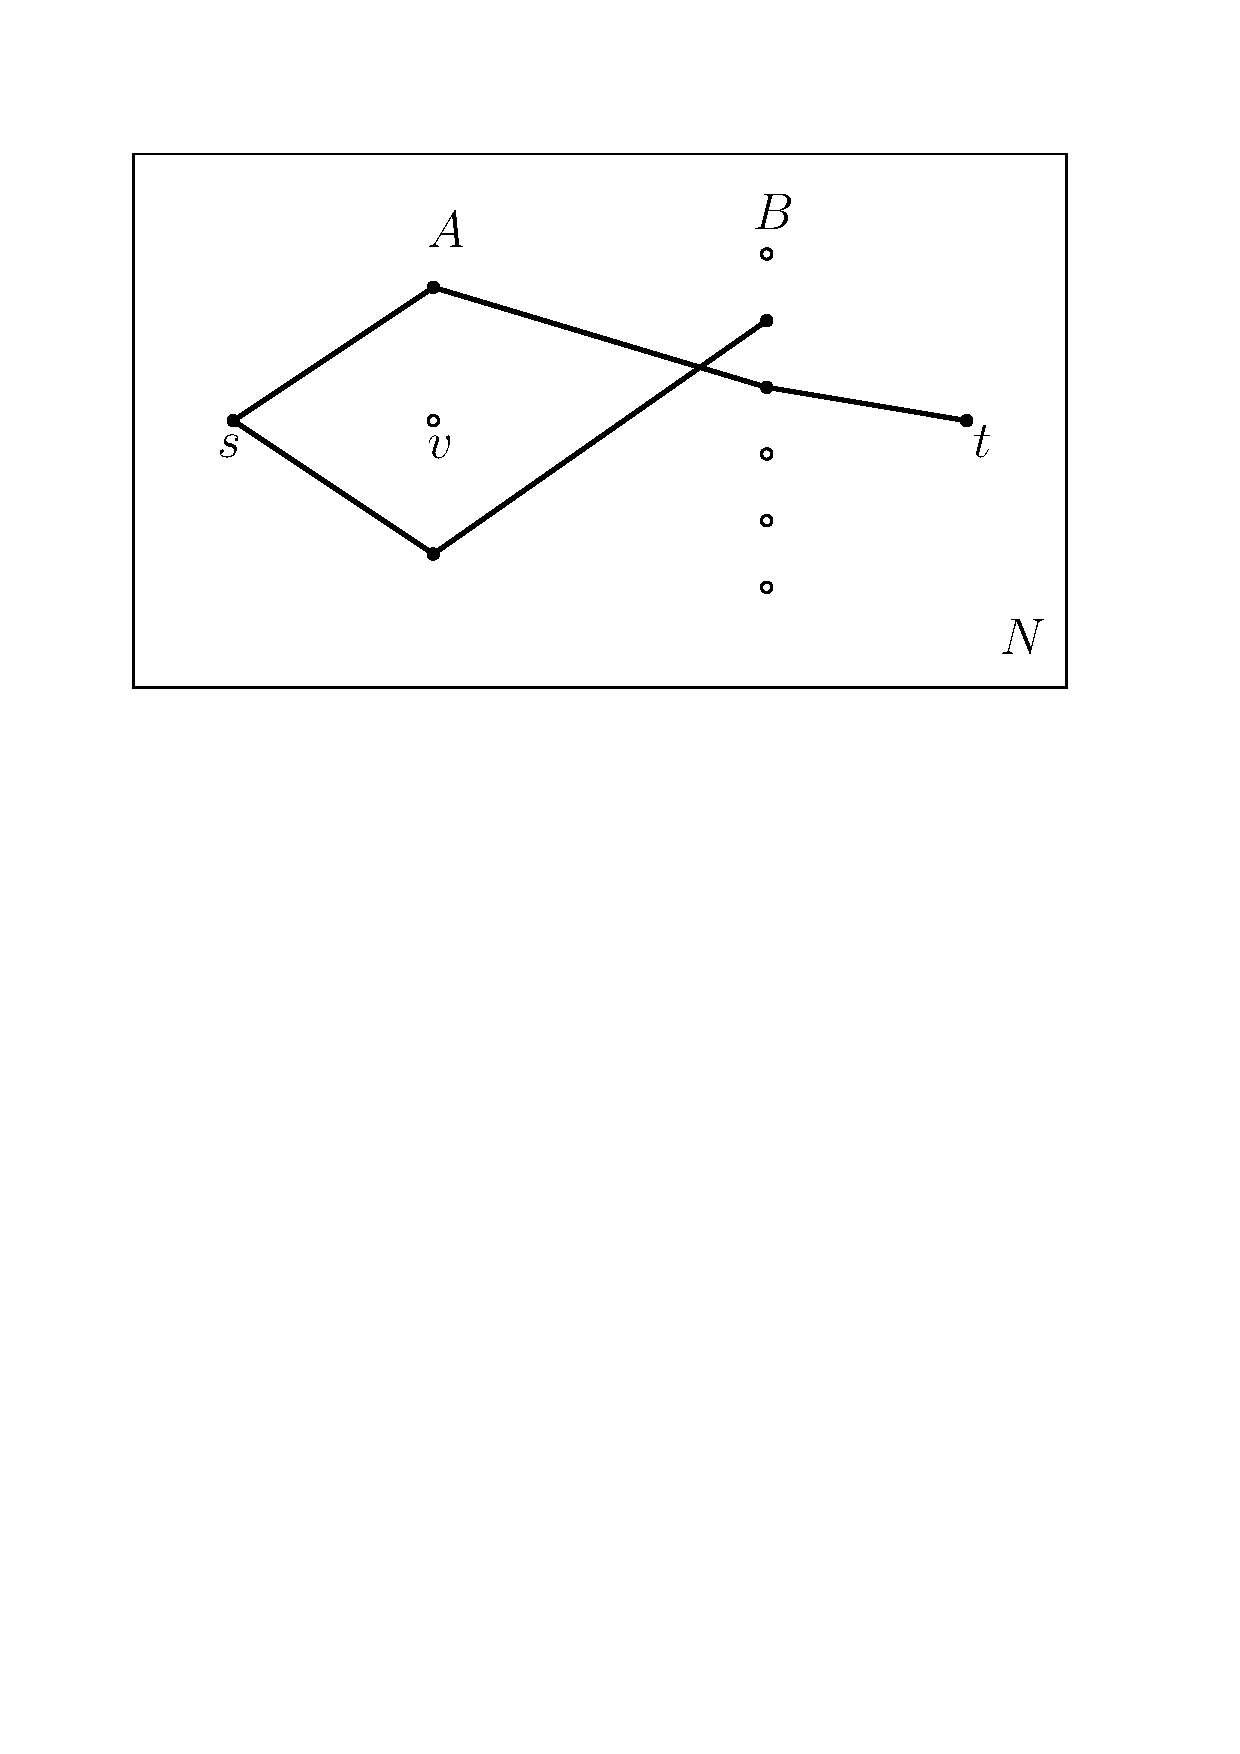
\includegraphics[width=0.3\textwidth,page=1]{shortcut.pdf}
\includegraphics[width=0.3\textwidth,page=2]{shortcut.pdf}
\includegraphics[width=0.3\textwidth,page=3]{shortcut.pdf}
\caption{
\label{fig:shortcut_network}
Shortcut network construction, with most arcs omitted for clarity.
Alive nodes are solid, dead nodes are hollow.
From left to right: support arcs of the current pseudoflow in bold,
the alive paths passing through dead node $v$,
and the shortcuts of these alive paths.
}
\end{figure}

\paragraph*{Correctness --- the shortcut network.}
\note{TODO figure, check the writing of this part} %TODO
Before continuing to describe potential updates, we prove that relaxing
alive paths keeps the Hungarian search intact.
Specifically, our process of relaxing alive paths in $N$ corresponds to
arc-by-arc relaxations in an equivalent (analysis-only) network we call the
\EMPH{shortcut network} $\tilde{N}$, ultimately creating a suitable potential.

The shortcut network is constructed from $N$ and $f$ as follows:
the nodes of $\tilde{N}$ are the alive nodes of $N$, and for each length-2, -3,
and forward length-1 alive path $\Pi = v \arcto \cdots \arcto w$ in $N$,
we add an arc $\arc vw$ in $\tilde{N}$ with $c(\arc vw) \gets c(\Pi)$.
This arc is the \EMPH{shortcut} of alive path $\Pi$, and denoted as \EMPH{$\short(\Pi)$}.
All arcs of $\supp(f)$ (in $N$) are themselves length-1 alive paths, so $f$
defines an identical pseudoflow on the shortcuts in $\tilde{N}$.
We abuse notation by using $f$ to refer to both the pseudoflow in $N$ as well as $\tilde{N}$.
With this, any excess-deficit path in $N_f$ can be mapped one-to-one to an
excess-deficit path in $\tilde{N}_f$ of the same cost, by mapping each alive
path in $N$ to its shortcut in $\tilde{N}$.
In fact, if we define potentials on the alive nodes, both paths will have
the same reduced cost (excess/deficit nodes are always alive).

As a result, a Hungarian search performing arc-by-arc relaxations on $\tilde{N}$
is equivalent to our process of relaxing alive paths in $N$.
For this to be helpful, the potential constructed on $\tilde{N}$ must produce
a useful potential for $N$.
The next lemma gives one such construction.

\begin{lemma}
\label{lemma:shortcut_correct}
For any $\theta$-optimal potential $\tilde{\pi}$ defined on $\tilde{N}$,
let $\pi$ be potential for $N$ constructed by extending $\tilde{\pi}$ to
dead nodes as follows:
\[
\pi(v) \gets \begin{cases}
	\tilde{\pi}(v) & v \in \alive{A} \cup \alive{B} \\
	\tilde{\pi}(s) & v \in \dead{A} \\
	\tilde{\pi}(t) & v \in \dead{B}
\end{cases}
\]
Then, $\pi$ is $\theta$-optimal for $N$, and if shortcut $\short(\Pi)$ is
admissible then the alive path $\Pi$ is also admissible.
\end{lemma}
\begin{proof}
We emphasize that the final statement is about arc-wise admissibility of $\Pi$,
and not its weak admissibility.
Indeed, even without extending $\tilde{\pi}$ to dead nodes, an admissible
$\short(\Pi)$ implies weak admissibility of $\Pi$ under $\tilde{\pi}$.

To prove the $\theta$-optimality of $\pi$, we need to check reduced costs of
length-2 and -3 alive paths, since it is immediate for length-1.
The analysis is nearly identical for both types of length-2 paths and length-3,
so we demonstrate it for alive paths of the form $s \arcto v \arcto b$ only.
For a length-2 alive path of the form $\Pi = s \arcto v \arcto b$,
for $b \in \alive{B}$, we have $c_\pi(\arc sv) = 0$ so we turn our eye to
the bipartite arc $\arc vb$.
Observe that the reduced cost of $\arc vb$, under $\pi$, is equal to the
reduced cost of $\short(\Pi)$ under $\tilde{\pi}$.
\begin{equation}
\label{eqn:shortcut_equiv}
\begin{aligned}
c_\pi(\arc vb) &= c(\arc vb) - \pi(v) + \pi(b) \\
	&= c(\Pi) - \pi(s) + \pi(b) \\
	&= c(\short(\Pi)) - \tilde{\pi}(s) + \tilde{\pi}(b) \\
	&= c_{\tilde{\pi}}(\short(\Pi))
\end{aligned}
\end{equation}
It follows that $\arc vb$ is $\theta$-optimal under $\pi$, by
$\theta$-optimality of $\short(\Pi)$ under $\tilde{\pi}$.
\[
c_\pi(\arc vb) = c_{\tilde{\pi}}(\short(\Pi)) \geq -\theta
\]

For the second statement, suppose a shortcut $\short(\Pi)$ is admissible.
Once again, the proof for each length is nearly identical, so we demonstrate
the proof only for $\Pi = s \arcto v \arcto b$.
The non-bipartite arc of $\Pi$ ($\arc sv$ with dead $v$) has reduced cost 0
under $\pi$; it is admissible.
By (\ref{eqn:shortcut_equiv}), admissibility of $\arc vb$ under $\pi$ follows
from admissibility of $\short(\Pi)$ under $\tilde{\pi}$.
\[
c_\pi(\arc vb) = c_{\tilde{\pi}}(\short(\Pi)) \leq 0
\]
Thus, all arcs of $\Pi$ are admissible, and $\Pi$ is admissible.
\end{proof}

\paragraph*{Updating potential.}
The query data structures for min-reduced-cost alive path have no dependency on
dead node potential; we leave them untracked as described before.
By Lemma~\ref{lemma:shortcut_correct}, a blocking flow supported on
weakly admissible alive paths is one that is arc-wise admissible ---
with the right extension of potential to dead nodes.
Indeed, we require values of $\pi$ on all nodes at the end of a scale
(for the next \textsc{Scale-Init}) and for individual dead nodes whenever they
become alive (after augmentation).
We use the construction in Lemma~\ref{lemma:shortcut_correct} to reconstruct a
potential for dead nodes in these situations.
Potential updates for alive nodes can be handled in a batched fashion as in
Section~\ref{section:hung}.

\paragraph*{Implementing the augmentation stage.}
\note{TODO check the writing of this part} %TODO
Augmentation can also be implemented in $O(k\polylog n)$ time, after
$O(n\polylog n)$ time preprocessing, using similar data structures.
The augmentation step finds an admissible blocking flow as a sequence of
disjoint admissible augmenting paths, using a depth-first search (DFS) through
the admissible residual arcs.
The DFS is initialized at each excess node and continues until it reaches a
deficit node with remaining deficit (an augmenting path is found),
or returns to the excess node (no path was found).
We attempt DFS from a new excess node once no path is found, or we have
found enough augmenting paths to balance the current excess.
In each step of the DFS, we discover admissible residual arcs by querying
the min-reduced-cost arc leaving the current node $x \in X$ into $V \setminus X$,
where $X$ is the set of excess nodes plus nodes already visited by the DFS.
If this minimum arc is admissible, we can search across it.
If it is not admissible, then there are no more unexplored admissible arcs
leaving $x$.
Like the Hungarian search, the DFS is reduced to a problem of querying the
min-reduced-cost arc.

Applying Lemma~\ref{lemma:shortcut_correct}, we can DFS through
weakly admissible alive paths instead of individual admissible arcs.
In implementation, we use data structures for dynamic \EMPH{nearest neighbor}
(NN) in addition to BCP.
The nearest neighbor problem is as follows:
preprocess a point set $P$ to answer, given a query point $a$, the point
$b \in P$ minimizing $c(a, b) - \omega(a) + \omega(b)$.
Kaplan~\etal~\cite{KMRSS17} solve the 2D dynamic NN problem with
$O(\polylog n)$ update and $O(\log^2 n)$ query time.
Similar to the Hungarian search implementation, we search across the
length-1, -2, and -3 alive paths that start at $x$.
Alive paths of the form $s \arcto v \arcto b$ and $s \arcto v \arcto w \arcto t$ are
still queried using BCPs, while those of the form $a \arcto b$ and
$a \arcto v \arcto t$ use an NN query with query point $x = a$ instead.
The total number of min-heaps and NN data structures is $O(1)$, and therefore
rewinding for the augmentation data structures can be done in $O(k\polylog n)$
time given Lemma~\ref{lemma:cost_scale_count}.

\paragraph*{Bounding relaxations and blocking flow support size.}
The following lemma is crucial to the analysis of running time for the
Hungarian search and augmentation, bounding both the number of relaxations and
potential update/recovery operations.

\begin{lemma}
\label{lemma:cost_scale_count}
Both Hungarian search and augmentation stages explore $O(k)$ nodes,
and the blocking flow found in augmentation stage is incident to $O(k)$ nodes.
\end{lemma}
\begin{proof}
Both processes explore by adding $O(1)$ nodes to $X$ in each step,
including at least one alive node.
Since the number of alive nodes is $O(k)$, the number of explored nodes is $O(k)$.

For the second statement, recall that our blocking flow is a union of of path
flows along admissible augmenting paths.
Each path flow is composed of alive paths explored by the depth-first search
in the augmentation stage, of which there are $O(k)$.
Since each such alive path has $O(1)$ length, the number of incident nodes is $O(k)$.
\end{proof}

We thus obtain the following:

\begin{lemma}
\label{lemma:refine_iter_time}
After $O(n\polylog n)$ time preprocessing, each iteration of \textsc{Refine} can be
implemented in $O(k\polylog n)$ time.
\end{lemma}


% ----------------------------------------------------------------------------
\section{Transportation algorithm}
\label{section:orlin}

Given two point sets $A$ and $B$ in $\reals^2$ of sizes $r$ and $n$ respectively
and a supply-demand function $\tsupply: A \cup B \to \ints$
as defined in the introduction, we present an $O(rn^{3/2}\polylog n)$ time
algorithm for computing an optimal transport map between $A$ and $B$.
By applying this algorithm in the case of $r \leq \sqrt{n}$ and the one by
Agarwal \etal~\cite{AFPVX17arxiv} when $r > \sqrt{n}$, we prove Theorem~\ref{theorem:orlin}.
We use a standard reduction to the uncapacitated min-cost flow problem and use
Orlin's algorithm~\cite{O93} as well as some of
the ideas from Agarwal \etal~\cite{AFPVX17arxiv} for efficient implementation under the geometric settings.
We first present an overview of the algorithm and then describe its fast
implementation that achieves the desired running time.

\paragraph*{From transportation to circulation}
Given a transportation instance between point sets $A$ and $B$, we generate a
min-cost flow network $N$ as follows: add an arc $\arc ab$ for each $a \in A$ and $b \in B$,
and copy the transportation supply/demand function to use as the MCF supply/demand function $\fsupply$.
A circulation $f$ in $N$ directly corresponds to a transportation map $\tau$
of the same cost, by setting $\tau(v, w) = f(\arc vw)$ for all arcs.

\subsection{Overview of the algorithm}

Orlin's algorithm follows an excess-scaling paradigm and the primal-dual framework.
It maintains a \EMPH{scale parameter} $\Delta$, a flow function $f$, and
potential $\pi$ on the nodes.
Initially $\Delta$ is equal to the total supply, $f = 0$, and $\pi = 0$.
We fix a constant parameter $\alpha \in (0.5, 1)$.
A node $v$ is called \EMPH{active} if the magnitude of imbalance of $v$ is at least $\alpha\Delta$.
%$\fsupply_f(v) \geq \alpha\Delta$. \note{defined long time ago}
At each step, using the Hungarian search, the algorithm finds an admissible
excess-to-deficit path between active nodes in the residual network and pushes a flow
of amount $\Delta$ along this path.%
\footnote{Note that this augmentation may convert an excess node into a deficit node.}
Repeat the process until either active excess or deficit nodes are gone; when this happens, $\Delta$ is halved.
The sequence of augmentations with a fixed value of $\Delta$ is called an
\EMPH{excess scale}.

The algorithm also performs two preprocessing steps at the beginning of each excess scale.
First, if $f(\arc vw) \geq 3n\Delta$, $\arc vw$ is contracted to a single node $z$ with
$\fsupply(z) = \fsupply(v) + \fsupply(w)$.%
\footnote{Intuitively, $f(\arc vw)$ is so high that future scales cannot deplete
the flow on $\arc vw$.}
Second, if there are no active excess nodes and $f(\arc vw) = 0$ for every arc $\arc vw$, then $\Delta$
is aggresively lowered to $\max_v \fsupply(v)$.

When the algorithm terminates, an optimal circulation in the
contracted network is found.
\note{TODO include a description of the contraction details}
We use the algorithm described in Agarwal~\etal~\cite{AFPVX17arxiv} to recover
an optimal circulation for the original network in $O(n\polylog n)$ time.
Orlin showed that the algorithm terminates within $O(n\log n)$ scales and
performs a total of $O(n\log n)$ augmentations.
In the next subsection, we describe an algorithm that, after $O(n\polylog n)$ time
preprocessing,
%performs a Hungarian search
finds an admissible excess-to-deficit path
in $O(r\sqrt{n} \polylog n)$ amortized time.
Summing this cost over all augmentations, we obtain the desired running time.

\subsection{An efficient implementation}

Recall in the previous sections that we could bound the running time of the
Hungarian search by the size of $\supp(f)$.
Here, the number of active imbalanced nodes at any scale is $O(r)$, and the
length of an augmenting path is also $O(r)$.
Therefore one might hope to find an augmenting path in $O(r\polylog n)$ time,
by adapting the algorithms described in Sections~\ref{section:hung} and
\ref{section:goldberg}.
The challenge is that $\supp(f)$ may have $\Omega(n)$ size,
therefore an algorithm which runs in time proportional to the support size is no longer
sufficient.
Still, we manage to implement Hungarian search in time $O(r\sqrt{n}\polylog n)$,
by exploiting a few properties of $\supp(f)$ as described below.

We note that each arc of $\supp(f)$ is admissible with reduced cost $0$,
so we prioritize the relaxation of support arcs as soon as they arrive in
$X \times (V \setminus X)$, over the non-support arcs.
This strategy ensures the following crucial property.

\note{TODO reference the lemma/proof from arxiv instead} %TODO
\begin{lemma}
\label{lemma:supp_acyclic}
If the support arcs $\supp(f)$ are relaxed as soon as possible, $\supp(f)$ is acyclic.
\end{lemma}

Next, similar to Section~\ref{section:goldberg}, we call node $u$
\EMPH{alive} if (a) $u$ is an active imbalanced node or (b) if $u$ is incident to
an arc of $\supp(f)$; $u$ is \EMPH{dead} otherwise.
Unlike in Section~\ref{section:goldberg}, once a node becomes alive it cannot
be dead again.
Furthermore, a dead node may become alive only at the beginning of a scale
(after the value of $\Delta$ is reduced).
Also, an augmenting path cannot pass through a dead node.
Therefore, we can ignore all dead nodes during Hungarian search,
and update the set of alive/dead nodes at the beginning of a scale.
%For a subset of nodes $S$, we use $\alive{S}$ to denote
%the set of alive nodes in $S$. \note{move to front and remove the one here}

Let $\EMPH{$B^\star$} \subseteq \alive{B}$ be the set of nodes that are either (a) active
imbalanced nodes or (b) incident to \emph{exactly one} arc of $\supp(f)$.
Lemma~\ref{lemma:supp_acyclic} implies that $\alive{B} \setminus B^\star$ has size $O(r)$.
%
We can therefore find the min-reduced-cost arc between $X \cap \alive{A}$ and $\alive{B} \setminus (B^\star \cup X)$
using a BCP data structure as in Section~\ref{section:hung}, along with lazy
potential updates and the rewinding mechanism.
The total time spent by Hungarian search on the nodes of $\alive{B} \setminus B^\star$ will be $O(r\polylog n)$.
We subsequently focus on handling $B^\star$.

\paragraph*{Handling $B^\star$.}
We now describe how we query a min-reduced-cost arc between $X \cap \alive{A}$
and $B^\star \setminus X$.
Each node $b \in B^\star$ is incident to exactly one arc in
$\supp(f)$.
%(i.e., there is only one outgoing arc from $b$).
We partition these nodes into clusters depending on their unique neighbor in $N_f$.
That is, for a node $a \in \alive{A}$,
let $\EMPH{$B_a^\star$} \coloneqq \{b \in B^\star \mid {\arc ab} \in \supp(f)\}$.
We refer to $B_a^\star$ as the \EMPH{star} of $a$.

The crucial observation is that $a$ is the only node in $N_f$ reachable from
each $b \in B_a^\star$, so once the Hungarian search reaches a node of $B_a^\star$ and thus
$a$ (recall we prioritize relaxing support arcs), the Hungarian search need
not visit any other nodes of $B_a^\star$, as they will only lead to $a$.
Hence, as soon as one node of $B_a^\star$ is reached, all other nodes of $B_a^\star$ can be
discarded from further consideration.
Using this observation, we handle $B^\star$ as follows.

We classify each $a \in \alive{A}$ as \EMPH{light} or \EMPH{heavy}:
heavy if $\abs{B_a^\star} \geq \sqrt{n}$,
and light if $\abs{B_a^\star} \leq 2\sqrt{n}$.
Note that if $\sqrt{n} \leq \abs{B_a^\star} \leq 2\sqrt{n}$ then $a$ may be classified
as light or heavy.
We allow this flexibility to implement reclassification in a lazy manner.
Namely, a light node is reclassified as heavy once $\abs{B_a^\star} > 2\sqrt{n}$,
and a heavy node is reclassified as light once $\abs{B_a^\star} < \sqrt{n}$.
This scheme ensures that the star of $a$ has gone through at least $\sqrt{n}$
updates between two successive reclassifications,
and these updates will pay for the time spent in updating the data structure
when $a$ is re-classified.
%--- see below.

For each heavy node $a \in \alive{A} \setminus X$, we maintain a BCP data
structure between $B_a^\star$ and $X \cap \alive{A}$.
Next, for all light nodes in $\alive{A} \setminus X$, we collect their stars into
a single set $\EMPH{$B_<^\star$} \coloneqq \bigcup_{\text{$a$ light}} B_a^\star$.
We maintain one single BCP data structure between $B_<^\star$ and $\alive{A} \cap X$.
Thus, at most $r$ different BCP data structures are maintained for stars.

Using these data structures, we can compute and relax a min-reduced-cost arc $\arc vw$ between
$\alive{A} \cap X$ and $B^\star \setminus X$.
%Once some arc ${\arc vw}$ between $\alive{A} \cap X$ and $B^\star \setminus X$
If $w$ lies in some star $B_a^\star$, then we also add $a$ into $X$.
If $a$ is light, then we delete $B_a^\star$ from $B_<^\star$ and update the BCP data structure of $B_<^\star$.
If $a$ is heavy, then we stop querying the BCP data structure of $B_a^\star$ for the
remainder of the search.
Finally, since $a$ becomes part of $X$, $a$ is added to all $O(r)$ BCP data structures.
%
Recall that $r \leq \sqrt{n}$ by assumption.
Adding arc $\arc vw$ thus involves performing $O(\sqrt{n})$
insertion/deletion operations in various BCP data structures, thereby taking
$O(\sqrt{n}\polylog n)$ time.

\paragraph*{Putting it together.}
The following lemma bounds the running time of the Hungarian search.

\begin{lemma}
Assuming all BCP data structures are initialized correctly, the Hungarian search
terminates within $O(r)$ steps, and takes $O(r\sqrt{n}\polylog n)$ time.
\end{lemma}
\begin{proof}
\note{TODO} %TODO
\end{proof}

Once an augmenting path is found and the augmentation is performed, the set of
imbalanced nodes and the support arcs change.
We thus need to update the sets $B^\star$, $B_a^\star$s, and $B_<^\star$.
This can be accomplished in $O(r\polylog n)$ amortized time.
When we begin a new Hungarian search, we use the rewinding mechanism
to set various BCP data structures in the right initial state.
Finally, when we move from one scale to another, we also update the sets
$\alive{A}$ and $\alive{B}$.
\note{TODO details?} %TODO
Omitting all the details, we conclude the following.

\begin{lemma}
Each Hungarian search can be performed in $O(r\sqrt{n}\polylog n)$ time.
\end{lemma}

Since there are $O(n\log n)$ augmentations and the flow in the original network
can be recovered from that in the contracted network in $O(n\polylog n)$
time~\cite{AFPVX17arxiv}, the total running time of the algorithm is
$O(rn^{3/2}\polylog n)$, as claimed in Theorem~\ref{theorem:orlin}.


% Acknowledgment and Bibliography
\paragraph*{Acknowledgment.}
We thank Haim Kaplan for useful discussion and suggesting to use Goldberg~\etal~\cite{GHKT17} for our approximation algorithm.
%
{
\bibliographystyle{newuser}
\bibliography{ref}
}

\appendix

\end{document}

%%%%%%%%%%%%%%%%%%%%%%%%%%%%%%%%%%%%%%%%%%%%%%%%%%%%%%%%%%%%%%%%%%%%%%%%%%%%%%%%%%%%
